\section{Dataset Construction}

Creating a referring segmentation dataset for aerial imagery presents unique challenges, as existing aerial datasets lack the natural language referring expressions required for this task. While high-quality instance and semantic segmentation datasets exist for aerial imagery, they contain only categorical labels and spatial annotations without the descriptive language needed to train referring segmentation models. This chapter describes our systematic approach to transforming these existing datasets into a comprehensive referring segmentation resource through automated rule-based generation of referring expressions.

Our methodology addresses this gap by developing a programmatic system that analyzes spatial relationships, visual characteristics, and positional information to generate natural language descriptions for aerial objects. The process begins with established aerial datasets that provide different annotation paradigms, extracts meaningful spatial and visual features from these annotations, and applies rule-based logic to construct referring expressions that capture object relationships, positions, and visual properties. Additionally, we convert semantic segmentation data into instance-level annotations where appropriate, enabling unified treatment of discrete objects and continuous landscape features within a single referring segmentation framework.

Beyond rule-based expression generation, we further enhance the dataset through multimodal large language model fine-tuning. We leverage the generalization capabilities of open-source multimodal LLMs, which possess both advanced language understanding and vision processing capabilities, to create more natural and diverse referring expressions. Through fine-tuning a multimodal LLM specifically on the task of expression enhancement, we apply this enhanced model to the full extent of our rule-based dataset, more than doubling the number of expressions from the original rule-based generation and significantly increasing the linguistic diversity and naturalness of the referring expressions.

\subsection{Source Datasets}

\noindent The AERIAL-D dataset is constructed from two primary sources of aerial imagery with fundamentally different annotation paradigms. The iSAID dataset is an instance segmentation dataset providing high-resolution aerial images with precise boundaries for individual object instances across fifteen categories including ships, vehicles, planes, buildings, and infrastructure elements such as harbors and bridges. In contrast, the LoveDA dataset is a semantic segmentation dataset that captures land cover and land use patterns, providing pixel-level classification into categories such as buildings, water bodies, agricultural areas, forests, and barren land. These two datasets ensure comprehensive coverage of both discrete objects and continuous landscape features commonly encountered in aerial imagery analysis.


% Dataset sources table with images
\begin{table}[H]
\centering
\caption{Source Dataset Characteristics}
\label{tab:dataset_sources}
\begin{tabular}{@{}p{4cm}p{8cm}@{}}
\toprule
\multicolumn{2}{c}{\textbf{iSAID Dataset}} \\
\midrule
\raisebox{-0.5\height}{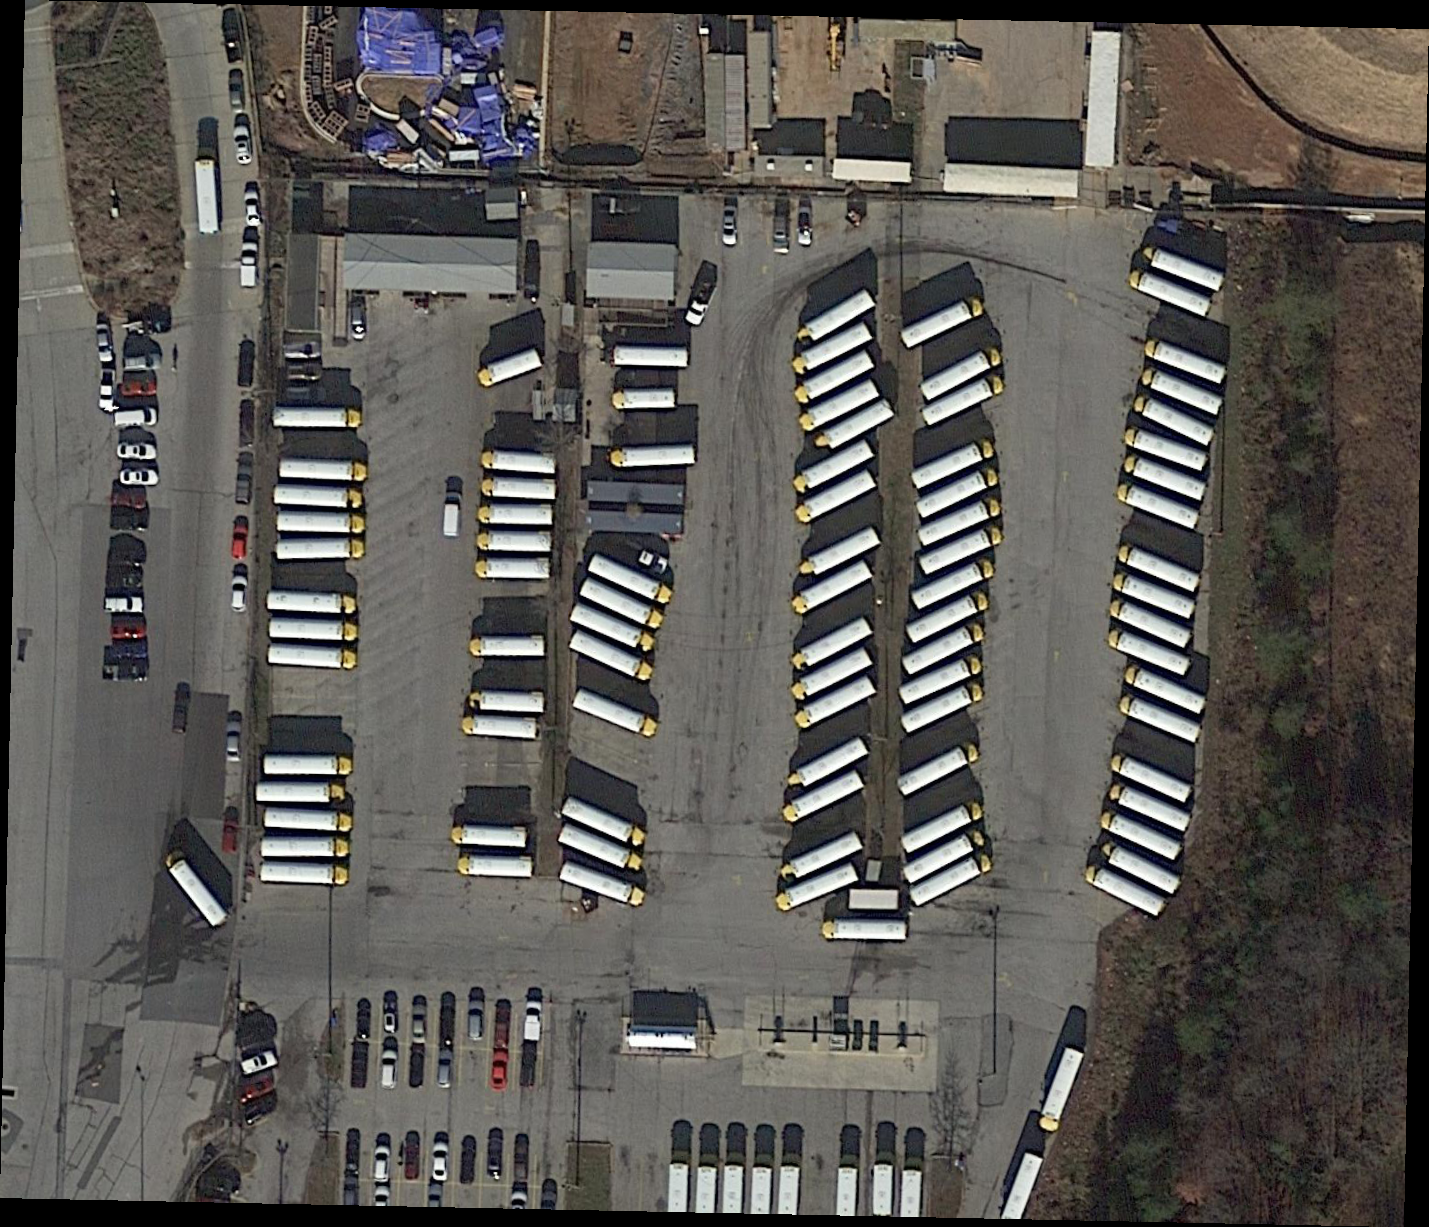
\includegraphics[width=3.5cm, height=3.5cm]{isaid.png}} & 
\hspace{-0.5cm}\parbox[c]{8cm}{\fontsize{10pt}{12pt}\selectfont Contains \textbf{2,806} high resolution images at varying widths of 800 to 13,000 pixels, spatial resolution of \textbf{0.1m to 4.5m}, with \textbf{655,451} instances across \textbf{15} object classes including \textbf{ships}, \textbf{large vehicles}, \textbf{small vehicles}, \textbf{planes}, etc.} \\[0.5cm]
\midrule
\multicolumn{2}{c}{\textbf{LoveDA Dataset}} \\
\midrule
\raisebox{-0.5\height}{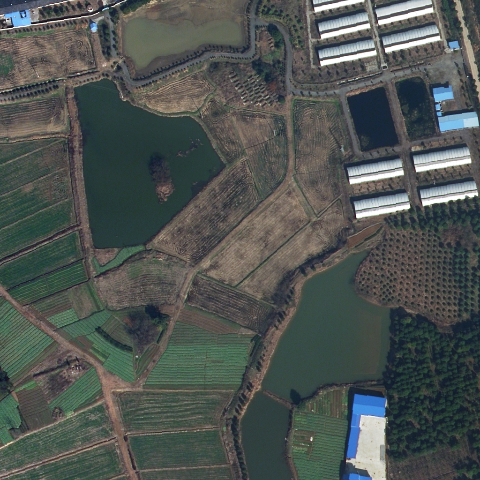
\includegraphics[width=3.5cm, height=3.5cm]{loveda.png}} & 
\hspace{-0.5cm}\parbox[c]{8cm}{\fontsize{10pt}{12pt}\selectfont Contains \textbf{5,987} images at 1024 pixel width, spatial resolution of \textbf{0.3m}, across \textbf{6} land cover classes: \textbf{building}, \textbf{road}, \textbf{water}, \textbf{barren}, \textbf{forest}, and \textbf{agriculture}.} \\[0.5cm]
\bottomrule
\end{tabular}
\end{table}



\subsection{Rule-Based Generation Pipeline}

\begin{figure}[H]
\centering
\begin{minipage}{0.5\textwidth}
\centering
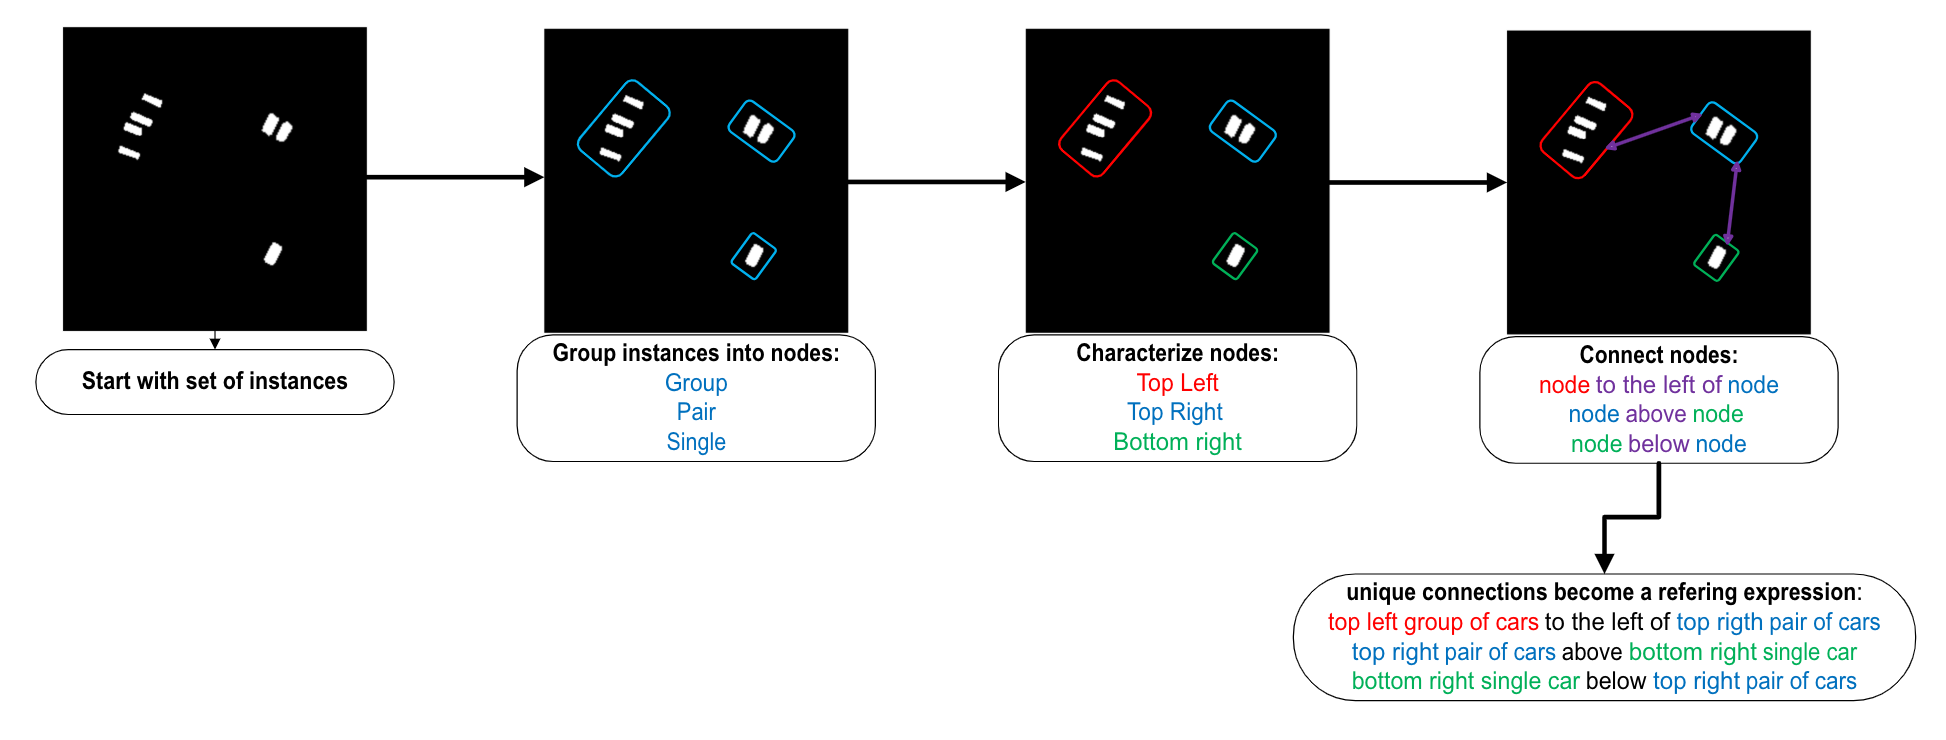
\includegraphics[width=0.7\textwidth]{rule_based_generation.png}
\end{minipage}%
\begin{minipage}{0.5\textwidth}
\centering
\hspace{-1cm}
\raisebox{-0.3\height}{%
\resizebox{\textwidth}{!}{%
\footnotesize
\begin{tabular}{@{}ll@{}}
\toprule
\textbf{Rule Type} & \textbf{Example Instance} \\
\midrule
Category & "plane" \\
Grid Position & "in the top right" \\
Extreme Position & None \\
Size Comparison & None \\
Color Classification & "light" \\
Directional Relations & "to the bottom right of a plane" \\
& "to the top right of a plane" \\
\midrule
\multicolumn{2}{l}{\textbf{Final Expressions}} \\
\multicolumn{2}{l}{"the plane in the top right"} \\
\multicolumn{2}{l}{"the light plane in the top right"} \\
\multicolumn{2}{l}{"the plane in the top right to the bottom right of a plane"} \\
\multicolumn{2}{l}{"the light plane in the top right to the bottom right of a plane"} \\
\multicolumn{2}{l}{"the plane in the top right to the top right of a plane"} \\
\multicolumn{2}{l}{"the light plane in the top right to the top right of a plane"} \\
\bottomrule
\end{tabular}%
}%
}
\end{minipage}
\caption{Example of rule generation for a single instance. The highlighted plane in the top right section demonstrates how the system assigns spatial, visual, and relational rules that will later be combined into referring expressions.}
\label{fig:rule_example}
\end{figure}

The rule-based generation pipeline transforms raw object annotations into structured linguistic descriptions through a comprehensive analysis of spatial, visual, and relational properties. This systematic approach ensures that every object instance receives detailed characterization across multiple dimensions, creating the foundation for diverse and contextually accurate referring expressions.

The pipeline begins by extracting fundamental metadata from each object instance, including category labels, precise bounding box coordinates, centroid positions, area measurements, and segmentation masks in run-length encoding format. A critical preprocessing step identifies partially visible objects through a cutoff flag, marking instances where less than half the object remains within the patch boundaries. This metadata serves as the foundation for all subsequent rule extraction and linguistic generation processes.

Spatial positioning forms the core structural element of the annotation system. Each image patch undergoes systematic partitioning into a three-by-three grid, establishing nine distinct spatial regions that provide consistent positional references. The system incorporates sophisticated borderline handling through a configurable center zone controlled by parameter alpha set to 0.2, creating a neutral area that helps resolve ambiguous boundary cases. When objects fall near grid cell boundaries, the system records both primary and alternative position labels, ensuring comprehensive coverage of spatial interpretations that later expand into multiple linguistic variants.

Extreme position detection operates independently within each object category, identifying instances that occupy the most prominent spatial positions along each axis. The system assigns topmost, bottommost, leftmost, and rightmost labels when the leading candidate maintains separation from the next closest instance by at least five percent of the total image extent along the corresponding dimension. This threshold ensures that extreme position assignments reflect genuinely distinctive spatial arrangements rather than minor positional variations.

Size-based characterization provides another crucial dimension for object differentiation. The system analyzes area measurements within each category to identify significant size outliers, applying a factor-of-1.5 separation rule to distinguish truly exceptional instances from normal size variations. Largest labels are assigned when an object's area exceeds the second-largest instance by this threshold, while smallest designations apply only to fully visible objects meeting the same separation criteria, preventing misleading size assessments based on partially occluded instances.

Relational analysis captures the complex spatial interactions between nearby objects through pairwise relationship computation. The system employs a dynamic proximity radius that combines a base distance value with size-dependent adjustments, ensuring that relationship detection scales appropriately with object dimensions. Directional analysis covers eight primary orientations including cardinal directions and diagonals, with sophisticated angular overlap detection using a 15-degree threshold to identify borderline cases where multiple directional interpretations remain valid. The system explicitly excludes containment relationships where one object's bounding box or centroid falls within another, focusing instead on meaningful spatial proximity relationships.

Group formation represents a higher-level organizational strategy that captures collective object arrangements. The system applies DBSCAN clustering algorithms independently within each object category, using minimum bounding box separation as the distance metric to identify natural object groupings. This approach produces meaningful multi-instance clusters while preventing oversized aggregations that would lose spatial coherence. Single-instance groups are created selectively, only when these isolated objects participate in relationships with established multi-instance groups, maintaining relational context across different scales of spatial organization.

Advanced grouping strategies extend beyond simple proximity clustering to capture semantic relationships. Class-level groups aggregate all instances of the same category within a patch, enabling expressions like "all buildings in the image" that refer to complete semantic sets. The system also recognizes special combination patterns, such as the pairing of small and large vehicles when both categories appear together, reflecting common real-world associations in aerial imagery.

Inter-group relationship analysis applies the same directional and proximity principles used for individual instances, but operates at the group level to capture higher-order spatial arrangements. The system computes relationships between multi-instance groups and between groups and individual instances, while avoiding redundant single-to-single relationships that are already captured at the instance level. This hierarchical approach enables complex referring expressions that reference both individual objects and their group affiliations.

Color analysis provides visual characterization through sophisticated pixel sampling and classification. The system extracts HSV color values from object segmentation masks, applying saturation thresholds to distinguish achromatic from chromatic colors and brightness analysis to separate light from dark variants. For chromatic colors, the system requires clear hue dominance before assignment, marking ambiguous cases where multiple color interpretations remain plausible. Domain-specific suppressions prevent inappropriate color assignments for certain categories like buildings and water bodies, where chromatic color variations typically result from imaging artifacts rather than meaningful visual properties.

The expression generation phase synthesizes comprehensive linguistic descriptions by systematically combining the extracted attributes. The system enumerates all valid combinations of category labels, grid positions, spatial relationships, extreme positions, size characteristics, and color properties. Borderline cases identified during attribute extraction expand into multiple expression variants, ensuring comprehensive coverage of alternative linguistic formulations. The system tracks expressions associated with cutoff objects or ambiguous color assignments as candidates for potential removal during final filtering.

Final processing ensures expression uniqueness and linguistic quality through systematic standardization and deduplication. The system normalizes category names and handles plural forms consistently, collapses single-instance groups into singular references, and removes any expression text that appears multiple times within a patch. This strict deduplication policy eliminates all occurrences of duplicated phrases, preventing ambiguous references that would compromise referring expression quality. Additional cleanup removes color expressions for objects with ambiguous color assignments, deletes objects and groups left without valid expressions, and removes entire patches that become empty after filtering. The final step strips intermediate rule fields from the XML annotations, producing clean datasets containing only unique, well-formed referring expressions.

% Expression uniqueness filter example
\begin{figure}[H]
\centering
\begin{minipage}{0.5\textwidth}
\centering
\includegraphics[width=0.7\textwidth]{filter_unique.png}
\end{minipage}%
\begin{minipage}{0.5\textwidth}
\centering
\hspace{-1cm}
\raisebox{-0.3\height}{%
\resizebox{\textwidth}{!}{%
\footnotesize
\begin{tabular}{@{}ll@{}}
\toprule
\textbf{Expression} & \textbf{Status} \\
\midrule
\multicolumn{2}{l}{\textbf{Object 1 (Light Vehicle)}} \\
\midrule
"the small vehicle in the top right" & \textcolor{red}{Filtered} \\
"the topmost small vehicle" & \textcolor{green}{Kept} \\
"the light small vehicle in the top right" & \textcolor{green}{Kept} \\
"the light topmost small vehicle" & \textcolor{green}{Kept} \\
"the small vehicle in the top right above a small vehicle" & \textcolor{green}{Kept} \\
\midrule
\multicolumn{2}{l}{\textbf{Object 2 (Dark Vehicle)}} \\
\midrule
"the small vehicle in the top right" & \textcolor{red}{Filtered} \\
"the dark small vehicle in the top right" & \textcolor{green}{Kept} \\
"the small vehicle in the top right below a small vehicle" & \textcolor{green}{Kept} \\
\bottomrule
\end{tabular}%
}%
}
\end{minipage}
\caption{Example of expression uniqueness filtering showing how ambiguous expressions are removed when multiple objects occupy similar spatial positions. The blue and red boxes highlight two small vehicles in the top right corner that would create conflicting references.}
\label{fig:uniqueness_filter}
\end{figure}

% Expression taxonomy table
\begin{table}[H]
\centering
\caption{Complete Taxonomy of Generated Expression Types}
\label{tab:expression_types}
\resizebox{\textwidth}{!}{%
\begin{tabular}{@{}ccccccl@{}}
\toprule
\textbf{Category} & \textbf{Position} & \textbf{Extreme} & \textbf{Size} & \textbf{Color} & \textbf{Relationship} & \textbf{Example} \\
\midrule
\multicolumn{7}{l}{\textbf{Individual Instance Expressions}} \\
\midrule
\checkmark & & & & & & "the ship" \\
\checkmark & \checkmark & & & & & "the ship in the bottom right" \\
\checkmark & \checkmark & & & & \checkmark & "the ship in the bottom right that is to the left of a harbor" \\
\checkmark & & \checkmark & & & & "the topmost ship" \\
\checkmark & \checkmark & \checkmark & & & & "the topmost ship in the top left" \\
\checkmark & \checkmark & \checkmark & & & \checkmark & "the topmost ship in the top left that is above a building" \\
\checkmark & \checkmark & & \checkmark & & & "the largest ship in the bottom right" \\
\checkmark & \checkmark & & \checkmark & & \checkmark & "the largest ship in the bottom right that is above a harbor" \\
\checkmark & \checkmark & \checkmark & \checkmark & & & "the largest topmost ship in the top left" \\
\checkmark & \checkmark & \checkmark & \checkmark & & \checkmark & "the largest topmost ship in the top left that is above a building" \\
\checkmark & & & & \checkmark & & "the dark ship" \\
\checkmark & \checkmark & & & \checkmark & & "the dark ship in the bottom right" \\
\checkmark & \checkmark & & & \checkmark & \checkmark & "the dark ship in the bottom right that is to the left of a harbor" \\
\checkmark & & \checkmark & & \checkmark & & "the dark topmost ship" \\
\checkmark & \checkmark & \checkmark & & \checkmark & & "the dark topmost ship in the top left" \\
\checkmark & \checkmark & \checkmark & & \checkmark & \checkmark & "the dark topmost ship in the top left that is above a building" \\
\checkmark & \checkmark & & \checkmark & \checkmark & & "the dark largest ship in the bottom right" \\
\checkmark & \checkmark & & \checkmark & \checkmark & \checkmark & "the dark largest ship in the bottom right that is above a harbor" \\
\checkmark & \checkmark & \checkmark & \checkmark & \checkmark & & "the dark largest topmost ship in the top left" \\
\checkmark & \checkmark & \checkmark & \checkmark & \checkmark & \checkmark & "the dark largest topmost ship in the top left that is above a building" \\
\midrule
\multicolumn{7}{l}{\textbf{Group Expressions}} \\
\midrule
\checkmark & \checkmark & & & & & "the group of 3 ships in the center" \\
\checkmark & \checkmark & \checkmark & & & & "the topmost group of 3 ships in the center" \\
\checkmark & \checkmark & & & & \checkmark & "the group of 3 ships in the center that is above a group of 2 buildings" \\
\checkmark & \checkmark & & & & \checkmark & "the ship in the bottom right that is to the left of a group of 2 harbors" \\
\checkmark & & & & & & "all buildings in the image" \\
\checkmark & & & & & & "all small and large vehicles in the image" \\
\bottomrule
\end{tabular}%
}
\end{table}

\subsection{LLM Enhancement Component}

% LLM enhancement example figure
\begin{figure}[H]
\centering
\begin{minipage}{0.5\textwidth}
\centering
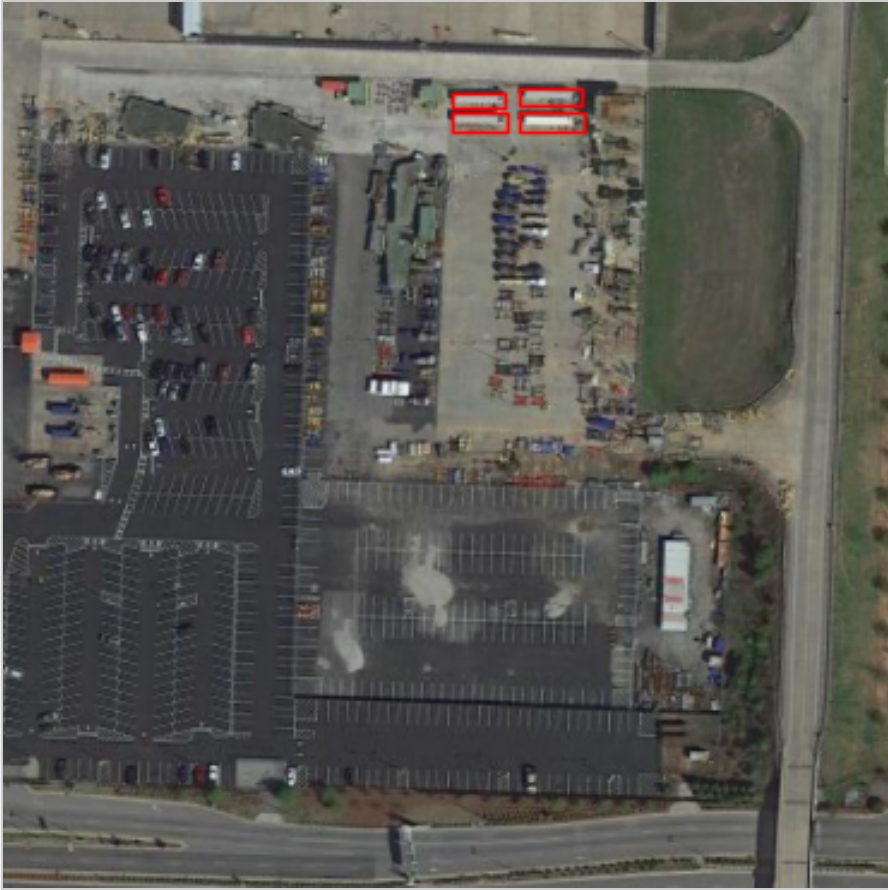
\includegraphics[width=0.7\textwidth]{example_group.png}
\end{minipage}%
\begin{minipage}{0.5\textwidth}
\centering
\hspace{-1cm}
\raisebox{-0.3\height}{%
\footnotesize
\begin{tabular}{@{}p{2cm}p{5cm}@{}}
\toprule
\textbf{Expression Type} & \textbf{Example} \\
\midrule
Original & the group of 4 large vehicles in the top center \\
\midrule
Enhanced & the cluster of four big vehicles near the upper middle \\
\midrule
Unique & the four large vehicles lined up side by side just below the pale paved strip at the very top middle \\
\midrule
Unique & the set of four big vehicles parked in a single row in the upper center beside the grassy area to the right \\
\bottomrule
\end{tabular}%
}
\end{minipage}
\caption{Example of LLM enhancement process showing original aerial image with group of four large vehicles (left) and corresponding expression enhancements (right).}
\label{fig:llm_enhancement_example}
\end{figure}


